\section{Execution Plan Generation}
\label{sec:queryPro}

Having illustrated the intended execution of an example program, we
now describe the steps required to automatically generate an execution plan from a
\Dlog program. We first focus on generating
an execution plan in a centralized implementation, before extending
the techniques to the network scenario.

\subsection{Centralized Plan Generation}
\label{sec:semiNaive}

In generating the centralized plan, we utilize the well-known {\em
  semi-\naive fixpoint}~\cite{semi,semi1} evaluation mechanism that
ensures no redundant evaluations. As a quick review, in semi-\naive (SN) evaluation, input
  tuples computed in the previous iteration of a recursive rule
  execution are used as input in the current iteration to compute
  new tuples. Any new tuples that are generated for the first time in the current
  iteration are then used as input to the next iteration. This is repeated until a
  fixpoint is achieved (\ie no new tuples are produced).

The semi-\naive rewritten rule for rule SP2 is shown below:

\vspace{2pt}
{\small
\noindent{\bf SP2-1: } $\triangle$path$^{new}$({\bf @S},@D,@Z,P,C) :- \link({{\bf @S},@Z},C$_{1}$),\\
\datalogspace
$\triangle$path$^{old}$({\bf @Z},@D,@Z$_{2}$,P$_{2}$,C$_{2}$), C = C$_{1}$ + C$_{2}$, \\                              
\datalogspace P =
$f\_concatPath$(link({{\bf @S},@Z},C$_{1}$),P$_{2}$).\\ 
}

\vspace{2pt}


%SP2-1* takes as input paths ($\triangle$path$^{old}$) computed in the previous
%invocation of the rule (known as an {\em iteration}), and use that to
%compute new paths ($\triangle$path$^{new}$). 


%Since links can also be modified during query execution, we need a
%similar rewrite for links (SP2-2). 

%{\small
%\noindent{\bf SP2-2: } $\triangle$path$^{new}$({\bf @S},@Z,@D,P,C) :-
%$\triangle$link({{\bf @Z},@S},C$_{1}$),\\
%\datalogspace path({\bf @Z},@D,@N,P$_{2}$,C$_{2}$), C = C$_{1}$ + C$_{2}$, \\                              
%\datalogspace P = $f\_concatPath$(linkD({\bf @Z},@S,C$_{1}$),P$_{2}$).\\ 
%}


\begin{figure*}[ht]
\centering
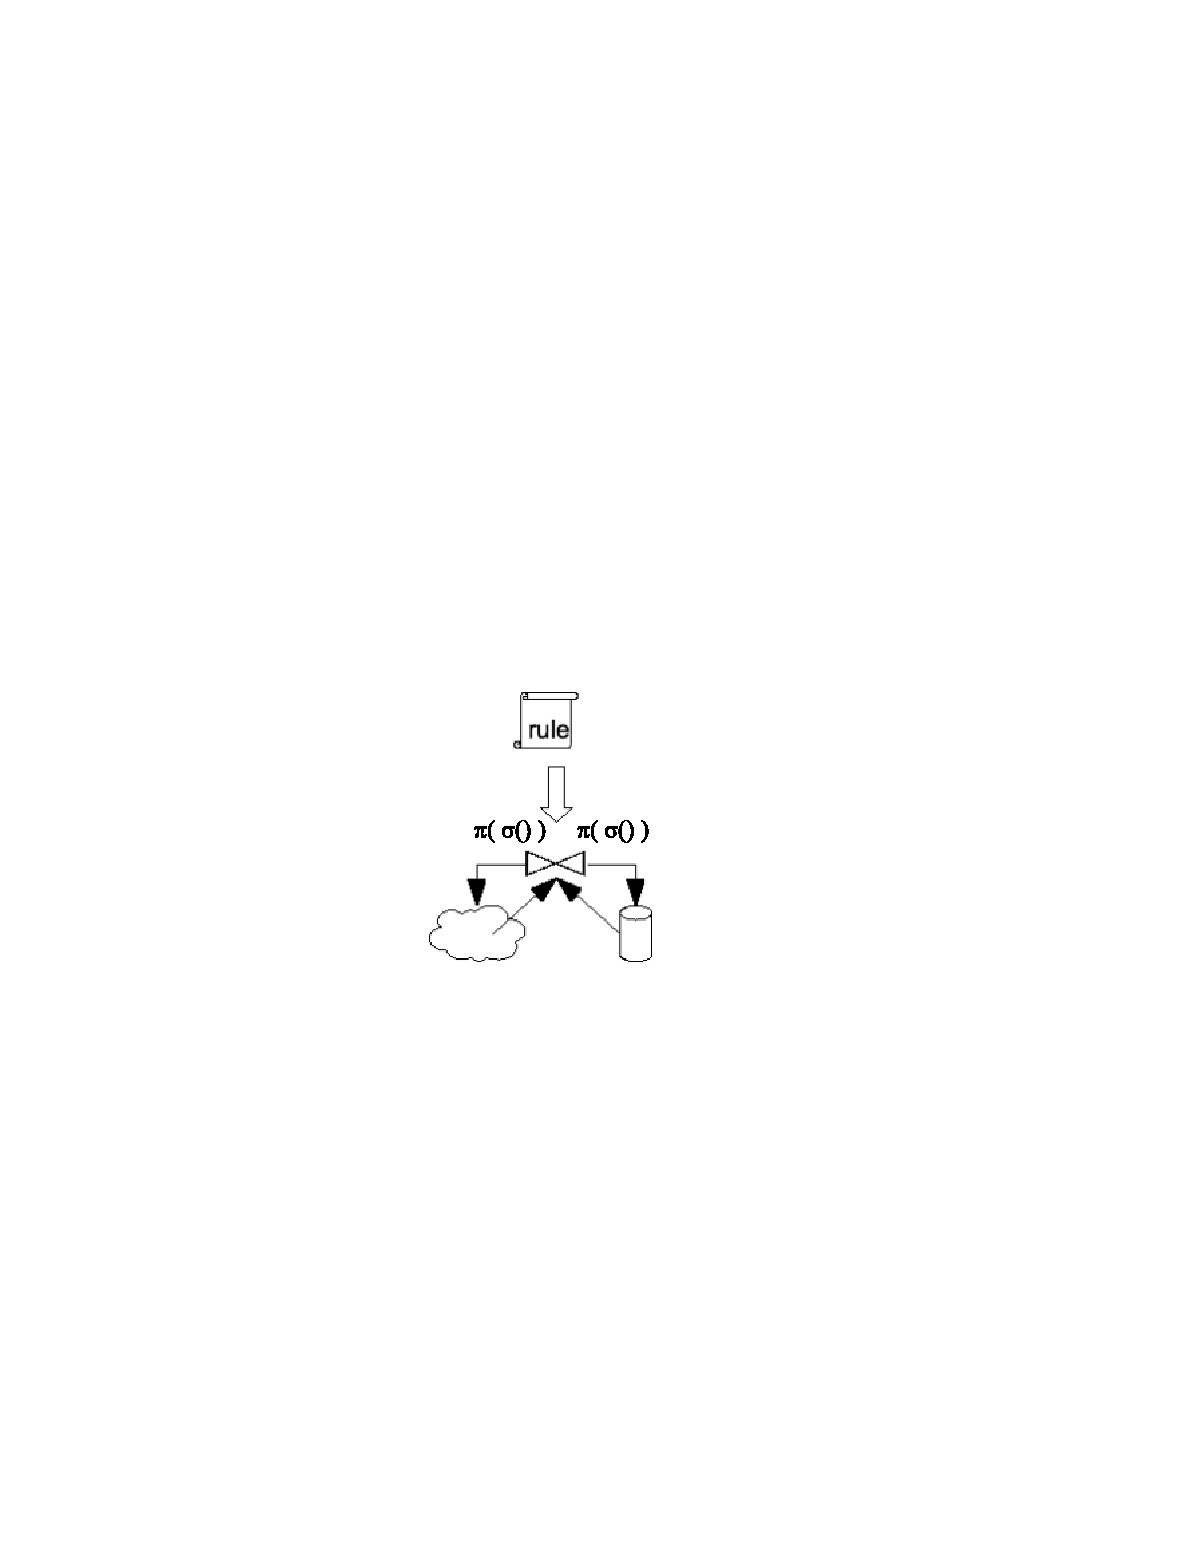
\epsfig{file=images/dataflow.eps, width=5in}
\caption{\label{Dataflow}\emph{\small Rule strand for rule SP2-1 in
    \Sys. Output paths that are generated from the strand are ``wrapped
    back'' as input into the same strand. }}
\end{figure*}                                        

Figure~\ref{Dataflow} shows the dataflow realization for rule SP2-1
using the conventions of \Sys. We will briefly explain how the semi-\naive evaluation is
achieved here. Each semi-\naive rule is implemented as a {\em rule strand}. Each strand
consists of a number of relational operators. The example strand
receives new $\triangle$$path^{old}$ tuples generated in the previous
iteration to generate new paths ($\triangle$$path^{new}$) which are
then inserted into the $path$ table (with duplicate elimination) for
further processing in the next iteration. 

In Algorithm~\ref{alg:sn}, we show the pseudocode for a centralized
\Sys implementation of multiple semi-\naive
rule strands where each rule has the form $\triangle$p$^{new}_{j}$ :-
$p^{old}_{1}$,..., $p^{old}_{k-1}$,$\triangle$p$^{old}_{k}$,$p_{k+1}$,...,$p_{n},b_{1},
b_{2},...,b_{m}$;\footnote{These rules are logically equivalent to rules
  of the form $\triangle$p$^{new}_{j}$ :- $p_{1},p_{2}$,...,$p_{k-1}$,$\triangle$p$^{old}_{k}$,$p_{k+1}$,...,$p_{n},b_{1},b_{2},...,b_{m}$,
  and have the advantage of avoiding redundant inferences within each iteration.}
\\$p_{1},...,p_{n}$ are recursive predicates and $b_{1},...b_{m}$ are base
predicates. $\triangle$p$^{old}_{k}$ refers to $p_{k}$ tuples generated
for the first time in the previous iteration. $p^{old}_{k}$
refers to all $p_{k}$ tuples generated before the previous iteration.

%|\quad | \triangle 
\vspace{2pt}
\begin{Algorithm}[ht]
  \begin{programbox}
%    |Initialize all | p_{i} | and | \triangle p^{new}_{i} to | null |
    \WHILE \exists B_{k}.size > 0
     \forall B_{k} | where | B_{k}.size > 0, \triangle p^{old}_{k} \leftarrow B_{k}.flush()
	|execute all rule strands | 	
	\FOREACH | recursive predicate | p_{j} 
	  p^{old}_{j} \leftarrow p^{old}_{j} \union \triangle p^{old}_{j}
	  B_{j} \leftarrow \triangle p^{new}_{j} - p^{old}_{j}
	  p_{j} \leftarrow p^{old}_{j} \union B_{j}
	  \triangle p^{new}_{j} \leftarrow \emptyset
%	\END
%    \END	      
\end{programbox}
\caption{Semi-\naive (SN) Evaluation in \Sys}
\label{alg:sn}
\end{Algorithm}
%end{boxedminipage}
\vspace{2pt}

In the algorithm, $B_{k}$ denotes the buffer for $p_{k}$ tuples
generated in the previous iteration
($\triangle$$p^{old}_{k}$). Initially, $p_{k}$, $p^{old}_{k}$, $\triangle$$p^{old}_{k}$ and
$\triangle$$p^{new}_{k}$ are empty. As a base case, we
execute all the rules to generate the initial $p_{k}$ tuples, which
are inserted into the corresponding $B_{k}$ buffers.  Each subsequent
iteration of the while loop consists of flushing all
existing $\triangle$$p^{old}_{k}$ tuples from $B_{k}$ and executing all
rule strands to generate $\triangle$$p^{new}_{j}$ tuples, which are used
to update $p^{old}_{j}$, $B_{j}$ and $p_{j}$ accordingly. Note that only new $p_{j}$ tuples
generated in the current iteration are inserted into $B_{j}$ for use in
the next iteration. Fixpoint is reached when all buffers are empty.
 
\subsection{Distributed Plan Generation}
\label{subsec:ruleLocalization}

In the distributed implementation of the {\em shortest-path} query,
non-local rules whose body predicates have different location
specifiers cannot be executed at a single node, since the tuples that
must be joined are situated at different nodes in the network. A {\em
  rule localization} rewrite step ensures that all tuples to be joined
are at the same node. This
allows a rule body to be locally computable.

%This step requires
%determining a distributed join ordering for predicates at different
%locations. 


\begin{figure}[ht]
\centering
\includegraphics[width=2.5in]{images/reachable.eps}
\caption{\label{Right Reachable}\emph{\small Logical Query Plan for rule SP2 from Section~\ref{sec:queryModel}.}}
\end{figure}                                              

Consider rule SP2 from Section~\ref{sec:queryModel}
where the link and path predicates have different location specifiers. These two
predicates are joined by a common ``@Z'' address
field. Figure~\ref{Right Reachable} shows the corresponding logical
query plan depicting the distributed join. The clouds represent an
``exchange''-like operator~\cite{volcano} that forwards tuples from one
network node to another; clouds are labeled with the link attribute that
determines the tuple's recipient. The
first cloud (\link.@Z) sends link tuples to the neighbor nodes indicated by their
destination address fields, %in order 
to join with matching path
tuples stored by their source address fields. The second cloud
($path.@S$) transmits for further processing new path tuples computed
from the join, setting the recipient according to the source address field.

Based on the above distributed join, rule SP2 can be rewritten into
the following two rules. Note that all
predicates in the body of SP2a have the same location specifiers;
the same is true of SP2b.


%\begin{figure}[ht]
%\begin{boxedminipage}{3.5in}
\vspace{2pt} 
{\small
\noindent{\bf SP2a: } linkD({\bf @Z},@S,C) :- \link({\bf @S},@Z,C).\\
{\bf SP2b: } path({\bf @S},@D,@Z,P,C) :- \link({\bf @Z},@S,C$_{3}$),linkD({\bf @Z},@S,C$_{1}$), \\
\datalogspace path({\bf @Z},@D,@Z$_{2}$,P$_{2}$,C$_{2}$),\\
\datalogspace C = C$_{1}$ + C$_{2}$, \\                              
\datalogspace P =
$f\_concatPath$(linkD({\bf @Z},@S,C$_{1}$),P$_{2}$).}
\vspace{2pt} 
%\end{boxedminipage}
%\small{\caption{\label{shortestPathLocal}\emph{\small Localized Rewrite for
%      rule SP2}}}
%\end{figure}

%{\bf FIXME: insert link restricted EXCHANGE~\cite{volcano} discussion}

%Rules SP2a and SP2b have the body predicates all at the
%same location.  
%In order to join matching link tuples and path
%tuples by the ``@Z'' field, link tuples are shipped by their destination
%addresses (as the $linkD$ message predicate) using rule SP2a. Rule SP2b then performs a join of the
%arriving linkD and path tuples. 

\begin{figure*}[ht]
\centering
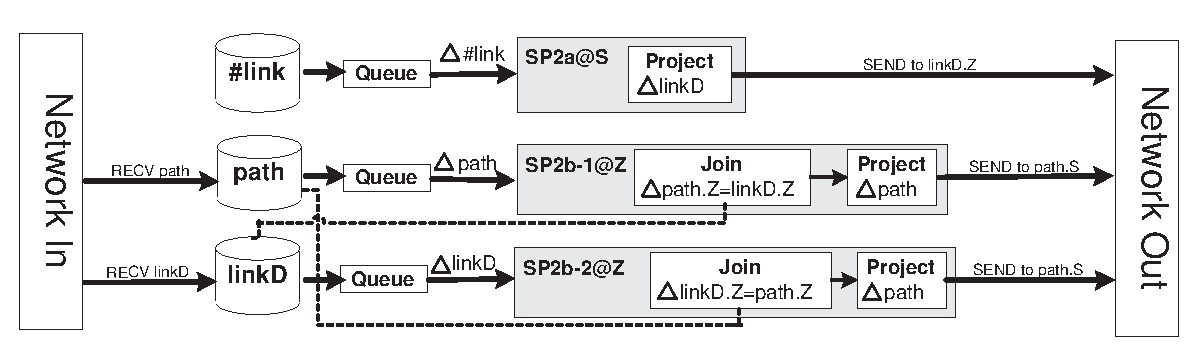
\epsfig{file=images/dataflow1.eps, width=5in}
\caption{\label{Dataflow1}\emph{\small Rule strands for the distributed
    version of SP2 after localization in \Sys.}}
\end{figure*}                                        

The rewrite is achievable because the $link$ and $path$ predicates,
although at different locations, share a common join address field. 
% Based
% on Definition~\ref{def:topRestricted}, we note that all
% link-restricted rules are localizable. 
In Algorithm~\ref{alg:ruleLocal}, we summarize the general rewrite
technique for an input set of link-restricted rules R. In the
pseudocode, for simplicity, we assume that the location specifiers of all the body
predicates are sorted (@S followed by @D); this can be done as a
preprocessing step. The algorithm as presented here assumes that all links are
bidirectional, and may add a \link(@D,@S) to a rewritten rule to
allow for backward propagation of messages.

\vspace{2pt}
{\scriptsize
\begin{Algorithm}[ht]
  \begin{programbox}
    \PROC |RuleLocalization| (R)
     \WHILE \exists | rule r |\in R|: |h(@L,...) :- |\link(@S,@D,...),|
     |\manyquads p|_{1}|(@S,..),..,p|_{i}|(@S,...),|
     |\manyquads p|_{i+1}|(@D,...),..,p|_{n}|(@D,..)| 
%     |\manyquads | \wedge | (| @L=@S | | \vee | | @L=@D )
            R.remove(r)	   
	    R.add(hS(@S,@D,..) :- |\link(@S,@D,..),..,p|_{i}|(@S,..).)|
	    R.add(hD(@D,@S,..) :- hS(@S,@D,..).)
	    \IF @L=@D 
	    \THEN R.add(|h(@D,..) :- hD(@D,@S,..),|
            |\manyquads p|_{i+1}|(@D,..),..,p|_{n}|(@D,..).|)
	    \ELSE R.add(|h(@S,..) :- \link(@D,@S),hD(@D,@S..),|
               |\manyquads p|_{i+1}|(@D,..),..,p|_{n}|(@D,..).|) 
%	       \IF \link.bidirectional
%	       | |\ELSE
%	       error(``illegal rule'')	       
%	       \FI
%            \FI
%     \END
%    \END      
\end{programbox}
\caption{Rule Localization Rewrite}
\label{alg:ruleLocal}
\end{Algorithm}
}
\vspace{2pt}

\begin{Claim}\label{claim:ruleLocal} Every link-restricted \Dlog program, when rewritten using
  Algorithm~\ref{alg:ruleLocal}, produces an equivalent program where
  the following holds:
\begin{CompactEnumerate}
\item The body of each rule can be evaluated at a single node.
\item The communication required to evaluate a rule is limited to
	sending derived tuples over links from a link relation.
\end{CompactEnumerate}
\end{Claim}

The equivalence statement in the above claim can be easily shown,
by examining the simple factoring of each removed rule into two parts. The
remainder of the claim can be verified syntactically in the added rules.
% 
%   because the algorithm generates rewritten
% rules whose body predicates have the same location specifier, and all
% non-local rules generates a tuple that is communicated forwards
% (\link(@S,@D)) or backwards (\link(@D,@S)) based on the input link
% predicate of the input rule. 


Returning to our example, after rule localization we perform the %
semi-\naive rewrite, and then generate the rule strands shown in
Figure~\ref{Dataflow1}.  Unlike the centralized strand in
Figure~\ref{Dataflow}, there are now three rule strands. The extra two
strands ({\em SP2a@S and SP2b-2@Z}) are used as follows. Rule strand
{\em SP2a@S} sends all existing links to the destination address field
as $linkD$ tuples.  Rule strand {\em SP2b-2@Z} takes the new $linkD$
tuples it received via the network and performs a join operation with
the local $path$ table to generate new paths.


\subsection{Relaxing Semi-\naive Evaluation}
In our distributed implementation, the execution of rule strands can
depend on tuples arriving via the network, and can also result in new
tuples being sent over the network. Traditional
semi-\naive evaluation completely evaluates all rules on a given set of
facts, \ie completes the {\em iteration}, before considering any new
facts.  In a distributed execution environment where
messages can be delayed or lost, the completion of an iteration in the
traditional sense can
only be detected by a consensus computation across multiple nodes,
which is expensive; further,
the requirement that many nodes complete the iteration
together (a ``barrier synchronization'' in parallel computing
terminology) limits parallelism significantly by restricting the rate
of progress to that of the slowest node.

We address this by making the notion of iteration local to a node.  New facts might
be generated through local rule execution, or might be received from another node
while a local iteration is in progress.
We propose and prove correct two variations of semi-\naive iteration
to handle this situation: {\em buffered
  semi-\naive} (BSN) and {\em pipelined semi-naive} (PSN).
  Both approaches extend SN to work in an
  asynchronous distributed setting, while generating the same
results as SN evaluation.
We further prove that these techniques avoid
duplicate inferences, which may result in generating network messages. 


\subsubsection{Buffered Semi-\naive}
{\em Buffered semi-\naive} (BSN) is the standard SN algorithm
described in Figure~\ref{alg:sn} with the following modifications: A node can
start a local SN iteration at any time its local $B_{k}$ buffers are
non-empty. Tuples arriving over the network while an iteration is in
progress are buffered for processing in the next iteration. 

By relaxing the need to run an iteration to global completion, BSN relaxes SN
substantially, by allowing a tuple from a traditional SN iteration to be
buffered arbitrarily, and handled in some future iteration of our choice. 
Consequently, BSN may generate
fewer tuples per iteration, but all results will eventually be
generated. Since BSN uses the basic SN
algorithm, the proof of correctness is straightforward and we omit it
for brevity.

The flexibility offered by BSN on when to process a tuple could also
be valuable outside the network setting, \eg a disk-based hash join
could accumulate certain tuples across iterations, spill them to disk in
value-based partitions, and process them in value batches, rather than
in order of iteration number.  Similar arguments for buffering apply
to other query processing tricks: achieving locality in B-tree
lookups, improving run-lengths in tournament sorts, etc.

\subsubsection{Pipelined Semi-\naive}
As an alternative to BSN, {\em pipelined semi-\naive} (PSN) 
relaxes semi-\naive evaluation to the extreme of processing each
tuple as it is received. This provides opportunities for additional
optimizations on a per-tuple basis, at the potential cost of set-oriented
local processing. New tuples that are generated from the
  semi-\naive rules, as well as tuples received from other nodes,
  are used immediately to compute new tuples 
without waiting for the current (local) iteration to complete. 

\vspace{2pt}
%begin{boxedminipage}{3in}
\begin{Algorithm}[ht]
  \begin{programbox}
    \WHILE \exists Q_{k}.size > 0
     t^{old,i}_{k} \LAR Q_{k}.dequeueTuple()
     \FOREACH | rule strand execution | 
     |\quad | \triangle p^{new,i+1}_{j} :- p_{1},..,p_{k-1},t^{old,i}_{k},p_{k+1},..,p_{n},b_{1},b_{2},...,b_{m}
       |\quad| \FOREACH  t^{new,i+1}_{j} \in \triangle p^{new,i+1}_{j}
         \IF t^{new,i+1}_{j} \notin p_{j} 
	 \THEN p_{j} \leftarrow p_{j} \union t^{new,i+1}_{j}
 	      Q_{j}.enqueueTuple(t^{new,i+1}_{j})
%	 \FI
%     \END      
%     \END
%   \END
\end{programbox}
\caption{Pipelined Semi-\naive (PSN) Evaluation}
\label{alg:psn}
\end{Algorithm}
%end{boxedminipage}
\vspace{2pt}


Algorithm~\ref{alg:psn} shows the pseudocode for PSN. Each tuple, denoted $t$, has a
  superscript ($old$/$new$, $i$) where $i$ is its corresponding iteration
  number in SN evaluation. Each processing step in PSN consists of dequeuing a
  tuple $t^{old,i}_{k}$ from $Q_{k}$ and then using it as input into all corresponding
  rule strands. Each resulting $t^{new,i+1}_{j}$ tuple is pipelined,
  stored in its respective $p_{j}$ table (if a copy is not already there), and enqueued into $Q_{j}$ for further
  processing. Note that in a distributed implementation, $Q_{j}$ can be
  a queue on another node, and the node that receives the new tuple can
  immediately process the tuple after the enqueue into $Q_{j}$. For example, the dataflow in Figure~\ref{Dataflow1}
  is based on a distributed implementation of PSN, where incoming
  $path$ and $linkD$ tuples received via the network are stored locally, and enqueued for
  processing in the corresponding rule strands.

%In
%  the pseudocode, each $Q_{k}$ is first initialized with the set
%  of $p_{k}$ tuples by running all the rules using the base tuples as
%  input. Subsequently, $Q_{k}$ acts as a buffer for new $p_{k}$ tuples. 

To fully pipeline evaluation, we have also removed the distinctions
between $p^{old}_{j}$ and $p_{j}$ in the rules. Instead, a timestamp (or
monotonically increasing sequence number) is added to each tuple at
arrival, and the join operator matches each tuple only  
with tuples that have the same or older timestamp. This allows processing of tuples immediately upon
arrival, and is natural for network message handling. This represents
an alternative ``book-keeping'' strategy to the rewriting used in SN to ensure no
repeated inferences. Note that the timestamp only needs to be assigned
locally, since all the rules are localized. 

While PSN enables fully pipeline evaluation, it is worth noting that PSN
can allow just as much buffering as BSN with the additional flexibility
of full pipelining.
%and also allows us to process the join operations on
%sets of tuples. 

%increasing sequence number (or timestamp) to each new tuple 
%prior to
%input to each join operator. Each tuple is then %


%Pipelining non-linear rules with multiple recursive predicates raises the complication of introducing
%duplicate inferences. Consider the following rule with $n$ recursive predicates and
%$m$ base predicates\\
%\noindent {\bf NL1:} $p :- p_{1}, p_{2}, ..., p_{n}, b_{1}, b_{2}, ..., b_{m}$

%In PSN evaluation, there are $n$ semi-\naive rules generated, one for
%each recursive predicate. For the $k^{th}$ recursive predicate, we
%define the {\em $k^{th}$ semi-\naive rule} as follows:\\
%\noindent {\bf NL1-k:} $\triangle$$p^{new} :- p_{1}, ..., \triangle$$p_{k}^{old}, ...,
%p_{n}, b_{1}, b_{2}, ..., b_{m}$

%Duplicates can arise when $t_{j} \in p_{j}$ and $t_{k} \in p_{k}$ are
%derived simultaneously. Based on the PSN algorithm, they are stored in
%their respective queues $Q_{j}$ and $Q_{k}$. When tuple $t_{j}$ is
%dequeued from $Q_{j}$, the $j^{th}$ rule is executed using the pair $t_{j}$
%and $t_{k}$ as inputs. Similarly, when tuple $t_{k}$ is dequeued, the
%pair is again used
%as input to the $j^{th}$ rule. %This results in repeated inferences.
 
In Appendix~\ref{appendix:pipeline}, we prove that PSN generates the same results as SN,
and does not repeat any inferences.
Let $FP_{S}(p)$ and $FP_{P}(p)$ denote the result set for $p$ for
using SN and PSN respectively. We show that:

\vspace{1pt}
\noindent{\bf Theorem~\ref{theorem:nonLinearEq}: } {\em $FP_{S}(p)=FP_{P}(p)$}\\
\noindent{\bf Theorem~\ref{theorem:dupnl}: } {\em There are no
  repeated inferences in computing $FP_{P}(p)$.} 
\vspace{1pt}

In order to compute rules with aggregation (such as SP3), we utilize incremental
fixpoint evaluation techniques~\cite{rossAggregate} that are amenable to
pipelined query processing. These techniques can compute {\em monotonic
  aggregates} such as $min$, $max$ and $count$
incrementally based on the current aggregate and each new input tuple. 
We omit the details for lack of space.



% for a general
%  semi-\naive rule  $\triangle$p$^{new,i+1}_{j}$ :-
%  $p_{1},..,p_{k-1},t^{old,i}_{k},p_{k+1},..,p_{n},b_{1},b_{2},...,b_{m}$. 

%The pseudocode above enforces tuple-at-a-time evaluation,
%which is computationally inefficient. As an optimization, we can flush
%the queue as before to perform set operations, and pipeline any
%generated tuples to their respective queues. 
%However, care has to be
%  taken to ensure that the iteration number is maintained correctly,
%  since the dequeued set may include tuples with different iteration
%  numbers. 




%However, enforcing the FIFO ordering in a queue is also necessary when
%  base tables are updated (Section~\ref{dynamic}).  

%In a distributed implementation of PSN, the queue ($Q$) corresponds to
%the input queue to the rule strand, and each node running the rule strand
%maintains its own separate queue. Hence, each $t^{new, i+1}_{1}$ tuple
%  generated can be inserted into a queue at another node.

%To illustrate PSN evaluation using the rule strands in Figure~\ref{Dataflow1}, we step through the
%communication necessary for the computing the path tuple 
%$p({\bf a},c,b,[a,c,b],2)$ for node {\em a} in Figure~\ref{SP
%  example}: 

%\vspace{1pt}

%\noindent {\bf $1^{st}$ iteration:} Node {\em a} sends
%  $link\_d({\bf a},c,1)$ to {\em c} ({\em rule strand SP2a@a}).

%\vspace{1pt}
%\noindent {\bf $2^{nd}$ iteration:} Node {\em c} receives
%  $link\_d({\bf c},a,1)$ and uses this tuple to 
%  $link\_d$ tuple is used to
%  perform the join ($\bowtie$) with
%  $path({\bf c},b,b,[c,b],1)$ to produce $path({\bf a},c,b,[a,c,d],2)$, which is sent back
%  to node {\em a} ({\em rule strand SP2b-2@c}). 

%\vspace{1pt}

%An optimization that we will explore later is a slight variant,
%known as {\em periodic pipelined} semi-\naive evaluation, where there is a fixed time-interval
%between iterations, and new tuples are processed in a set-oriented fashion.

%\subsubsection{PSN for Linear Rules}
%Consider the following semi-\naive rewritten rule from
%Section~\ref{sec:queryPro}:\\ 
%\noindent{\bf LR1a:} $\triangle$p$^{new}$ :- $\triangle$p$^{old}_{1}$,
%$b_{1}, b_{2}, ..., b_{m}$, where $p_{1}$ is a recursive predicate. 

%\vspace{2pt}
%\noindent{\bf Theorem~\ref{theorem:nseqpsn}: } {\em $FP_{S}(p) =
%FP_{P}(p)$.}\\
%\noindent{\bf Theorem~\ref{theorem:psnnodups}} {\em There are no
%  repeated inferences in computing $FP_{P}(p)$.} 
%\vspace{2pt}

%\subsubsection{PSN for Non-Linear Rules}



%As an optimization to pipelined evaluation, we can execute each rule strand periodically, by
%buffering up events in the queue, and then processing all events when a
%rule strand is activated. This is the pipelined semi-\naive evaluation
%described earlier.



